\documentclass[12pt,a4paper]{article}

% Language setting
\usepackage[british]{babel}

% Set page size and margins
\usepackage[a4paper,top=2cm,bottom=2cm,left=2.5cm,right=2.5cm,marginparwidth=1.75cm]{geometry}

%----------- APA style references & citations (starting) ---
% Useful packages
%\usepackage[natbibapa]{apacite} % APA-style citations.

\usepackage[style=apa, backend=biber]{biblatex} % APA 7th edition style citations using biblatex
\addbibresource{GPCO486.bib} % Your .bib file

% Formatting DOI in APA-7 style
%\renewcommand{\doiprefix}{https://doi.org/}

% Add additional APA 7th edition requirements
\DeclareLanguageMapping{british}{british-apa} % Set language mapping
\DeclareFieldFormat[article]{volume}{\apanum{#1}} % Format volume number

% Modify 'and' to '&' in the bibliography
\renewcommand*{\finalnamedelim}{%
  \ifnumgreater{\value{liststop}}{2}{\finalandcomma}{}%
  \addspace\&\space}
  
%----------- APA style references & citations (ending) ---


\usepackage{amsmath}
\usepackage{graphicx}
\usepackage[colorlinks=true, allcolors=blue]{hyperref}
\usepackage{hyperref}
\usepackage{orcidlink}
\usepackage[title]{appendix}
\usepackage{mathrsfs}
\usepackage{amsfonts}
\usepackage{booktabs} % For \toprule, \midrule, \botrule
\usepackage{caption}  % For \caption
\usepackage{threeparttable} % For table footnotes
\usepackage{algorithm}
\usepackage{algorithmicx}
\usepackage{algpseudocode}
\usepackage{listings}
\usepackage{enumitem}
\usepackage{chngcntr}
\usepackage{booktabs}
\usepackage{lipsum}
\usepackage{subcaption}
\usepackage{authblk}
\usepackage[T1]{fontenc}    % Font encoding
\usepackage{csquotes}       % Include csquotes
\usepackage{diagbox}


% Customize line spacing
\usepackage{setspace}
\doublespacing % 1 line spacing

% Redefine section and subsection numbering format
\usepackage{titlesec}
\titleformat{\section} % Redefine section numbering format
  {\normalfont\Large\bfseries}{\thesection.}{1em}{}
  
% Customize line numbering format to right-align line numbers
\usepackage{lineno} % Add the lineno package
\renewcommand\linenumberfont{\normalfont\scriptsize\sffamily\color{blue}}

% Define a new command for the fourth-level title.
\newcommand{\subsubsubsection}[1]{%
  \vspace{\baselineskip}% Add some space
  \noindent\textbf{#1\\}\quad% Adjust formatting as needed
}
% Change the position of the table caption above the table
\usepackage{float}   % for customizing caption position
\usepackage{caption} % for customizing caption format
\captionsetup[table]{position=top} % caption position for tables

% Define the unnumbered list
\makeatletter
\newenvironment{unlist}{%
  \begin{list}{}{%
    \setlength{\labelwidth}{0pt}%
    \setlength{\labelsep}{0pt}%
    \setlength{\leftmargin}{2em}%
    \setlength{\itemindent}{-2em}%
    \setlength{\topsep}{\medskipamount}%
    \setlength{\itemsep}{3pt}%
  }%
}{%
  \end{list}%
}
\makeatother

% Suppress the warning about \@parboxrestore
\pdfsuppresswarningpagegroup=1


%-------------------------------------------
% Paper Head
%-------------------------------------------
\title{How Does Nation State Choose Their Rivalry?}

\author[1]{Guanhao Hu}
\affil[1]{\small GPCO 486 Evaluating Technological Innovation}

\date{}  % Remove date

\begin{document}
\maketitle


\textbf{Keywords}: Regime Change, Foreign Policy Similarity, Interstate Dispute, Event Study

%-------------------------------------------
% Paper Body
%-------------------------------------------
%--- Section ---%
\section{Introduction}
What is the explicit threat signal that triggers a nation state engaging in a militarized interstate disputes? Apart from implicit system factors e.g., polarity and power distribution which can hardly observe the turning point across time for a country to perceive enough threats, regime change could be a more immediate threat to be identified. Meanwhile, it is less than enough for regime change to be the salient causal identification to explain where the militarized interstate disputes happen. For instance, when regime change both took place in Republic of China and Korean Peninsular, why the U.S. only engaged in the Korean War in a large scale instead of the Chinese Civil War. 
\\Therefore, I argue that together, regime change and foreign policy similarity also matters in terms of why the militarized interstate disputes happen in one dyad rather than the others. The main hypothesis in this research is that when regime change happens in a dyad set---nation state $i$ and nation state $j$---would more likely engage in a militarized interstate dispute if state $i$ shares less foreign policy similarity with state $j$. With the two-way way fixed effect regression and difference-in-differences which controls heterogeneity across time and individual, the main hypothesis would pass the test if a dyad undergoes regime change, the probability of militarized interstate dispute onsets increase significantly on average, in comparison to dyads would have not undergone regime change, with less similarity in foreign policy. 

\section{Research Design}
The causal identification of regime change's impact on the possibility of a militarized interstate dispute onset is addressed through the lens of non-directed analysis with dyad-year panel data. With that being said, in this research, directed relationship in a dyad---whether it involves the initiator or target of a militarized interstate dispute, regime change on either or both sides---is trivial. Since our unit of analysis is each dyad in each year and all research variables are non-directed and dyad-year, the causal effect of regime change on militarized interstate dispute onset is derived from variations among dyads instead of cross-sectional difference between nation state $i$ or nation state $j$. For instance, it is trivial to discuss, in this research, that how regime change which happens in initiator states would differ its effects on militarized interstate dispute onsets from which happens in target states. I focus on studying regime change in dyads and its effects on dyad's possibility to encounter a militarized interstate dispute.
\\Regarding the time span of this research, I only include observations from 1945 to 2010. Firstly, I have most of the observations of dyad-year regime change in mentioned time span. (see \ref{app1}) Secondly, the structural factor, polarity and power structural, is controlled in the time span and all dyads will be placed into bipolar system. Last but not least, the overlapped availability for all research variables from various data sets is within the above time span.
\subsection{Research Hypothesis}
\begin{center}
\begin{itemize}
\begin{itemize}
    \item $Hypothesis_1:$ Regime change leads dyads to be more likely to experience militarized interstate disputes.
\end{itemize}
\end{itemize}
\end{center}
First research hypothesis intends to gauge whether regime change is accountable as treatment effect in explaining changes in militarized interstate dispute onsets after either or both nation states in a dyad encounter the treatment.
\begin{center}
\begin{itemize}
\begin{itemize}
    \item $Hypothesis_2:$ Regime change leads dyads that shares high degress of foreign policy similarity to be more likely to experience militarized interstate disputes.
\end{itemize}
\end{itemize}
\end{center}
Furthermore, I argue that foreign policy similarity may have positive influence on nation state's decision to engage in a militarized interstate dispute with the other nation state that encounters regime change. Regime change could be a threat to other state's national security interests. Thus, nation states in highly similar dyads, in terms of their foreign policy preference profile, have more incentives to address their perception of threats and end up engaging in a militarized interstate disputes.

\subsection{Outcome Variable}
Militarized interstate dispute is coded as a dummy variable in non-directed dyad-year data set to indicate the onset. It records whether there is a militarized interstate dispute for a dyad in the given year. CoW MID Project (V5.0) provides conflicts data in which one or more states threaten, display, or use force against one or more other states between 1816 and 2014.\parencite{palmer_2021_the} 

\subsection{Explanatory Variables}
\begin{enumerate}
    \item Regime change is a dummy and non-directed variable. In any year, dyads would be recognized to have regime change if for either or both nation states, the duration of current regime existence turns into 0 and restarts to accumulate. Polity IV Projects (2018) records duration of each regime's survival at the year level. \parencite{marshall_2019_polity} Even though literature in democratic peace would argue that dyad's regime type (i.e., two democratic, two autocratic, democratic-autocratic and vice versa) matters in conflict study, such regime type consideration is excluded from our research since our analysis is only interested in non-directed results. \parencite{raknerud_1997_the} To decide the treatment year, I choose the initial year of the first either or both regime change observed in a dyad as the treatment year.
    \item Foreign policy similarity index is represented by Cohen's \textit{kappa} which is a coefficient meansured by dyad's Alliance preference profiles and weighted by squared distances. \parencite{hge_2011_choice, cohen_1960_a} High Cohen's \textit{kappa} indicates that the dyad has similar preference over choosing their Alliances and thus, they would have more similar foreign policy. Cohen's \textit{kappa} coefficients range from $-1$ to $1$ with $1$ indicating identical foreign policy preference for a dyad.
\end{enumerate}

\subsection{Control Variables}
\begin{enumerate}
    \item Strategic rivalry. A dummy variable indicates dyad's strategic rivalry relationship. It is defined according to the density of previous conflicts history. \parencite{thompson_2012_handbook}
    \item Alliance. CoW Formal Alliances (V4.1) data set defines four levels of Alliance relationships, i.e., defense pact, neutrality, non-aggression treaty, entente agreement. \parencite{gibler_2009_international} If a dyad includes any one of the four levels of Alliance relationship, the dyad would be regarded as having at least entente level of Alliance relationship.
    \item Major Power power. A dummy variable indicates at least one Major Power power is included in a dyad. CoW State System Membership (V2016) data set defines Major Power power from 1816 to 2016.
    \item Distance. The minimum distance between nation states on Jan. 1 of the year, in kilometers. \parencite{schvitz_2021_mapping}
    \item Trade. Sum of import amount (millions of current USD) between dyads. Then, calculate the Z-score of dyad's amount of import in each given year. Data from CoW Trade (V4.0). \parencite{barbieri_2009_trading}
    \item Economic Development. Aggregate of dyad's GDP per capita. (log-transformed in 2011 USD) Then, calculate the Z-score of the aggregate in each given year. \parencite{anders_2020_bread}
    \item National military capability. Dyad's difference in national military capability. The national capability ratio is calculated by obtaining the ratio of one nation state's Composite Index of National Capability Score compared to all the other nation states in the system. \parencite{singer_1988_reconstructing} Then, calculate the Z-score of that difference in each given year. Data from CoW National Material Capabilities (V6.0).
\end{enumerate}

\subsection{Statistical Model}
\begin{center}
        $MID_{(i,j)t} = \alpha_{i} + \alpha_{j}+ \lambda_{t} + \beta X_{(i,j)t} + \beta_1 T_{1(i,j)t} + \beta_2 x_{2(i,j)t} + \delta (T_{1(i,j)t} \times x_{2(i,j)t}) + \epsilon_{(i,j)t}$
\end{center}
The causal identification from this research focus on examining and interpreting $\beta_1$ as for treatment variable, regime change, and $\delta$ as for interactive effect that foreign policy similarity has on treatment effect. More specifically, the causal identification will be derived from: 
\begin{center}
    $\delta=E\{y_i|x_i,T_i=1\}-E\{y_i|x_i,T_i=0\}$
\end{center}
which is the average treatment effect (ATT) from the difference in the likelihood of a regime change dyad engaging in a militarized interstate dispute compared to what it would have been if it had not undergone the treatment. Indeed, dyadic fixed effects $\alpha_{i}$ and $\alpha_{j}$ from states $i$ and $j$ and time fixed effect $\lambda_{t}$ will be taken into account by the regression model.

\section{Statistical Analysis}
The effect size and minimum detected effect indicates that research has enough samples to continue the research. (see table~\ref{efsize} and figure~\ref{mde}) There are 1,000 unique dyads and 724,492 observations.
\\Since regime change is orthogonal to time, research data has staggered entry of the treatment. Cross-sectional difference among dyads may related to the timing of regime change. The cross-sectional test results in table~\ref{cset} confirm such endogeneity issue. However, the cross-sectional endogeneity issue will be resolved by Two-way Fixed Effect regression as cross-sectional fixed effect being controlled. 
\subsection{Parallel Trend Analysis}
\begin{figure}[!ht]
\centering
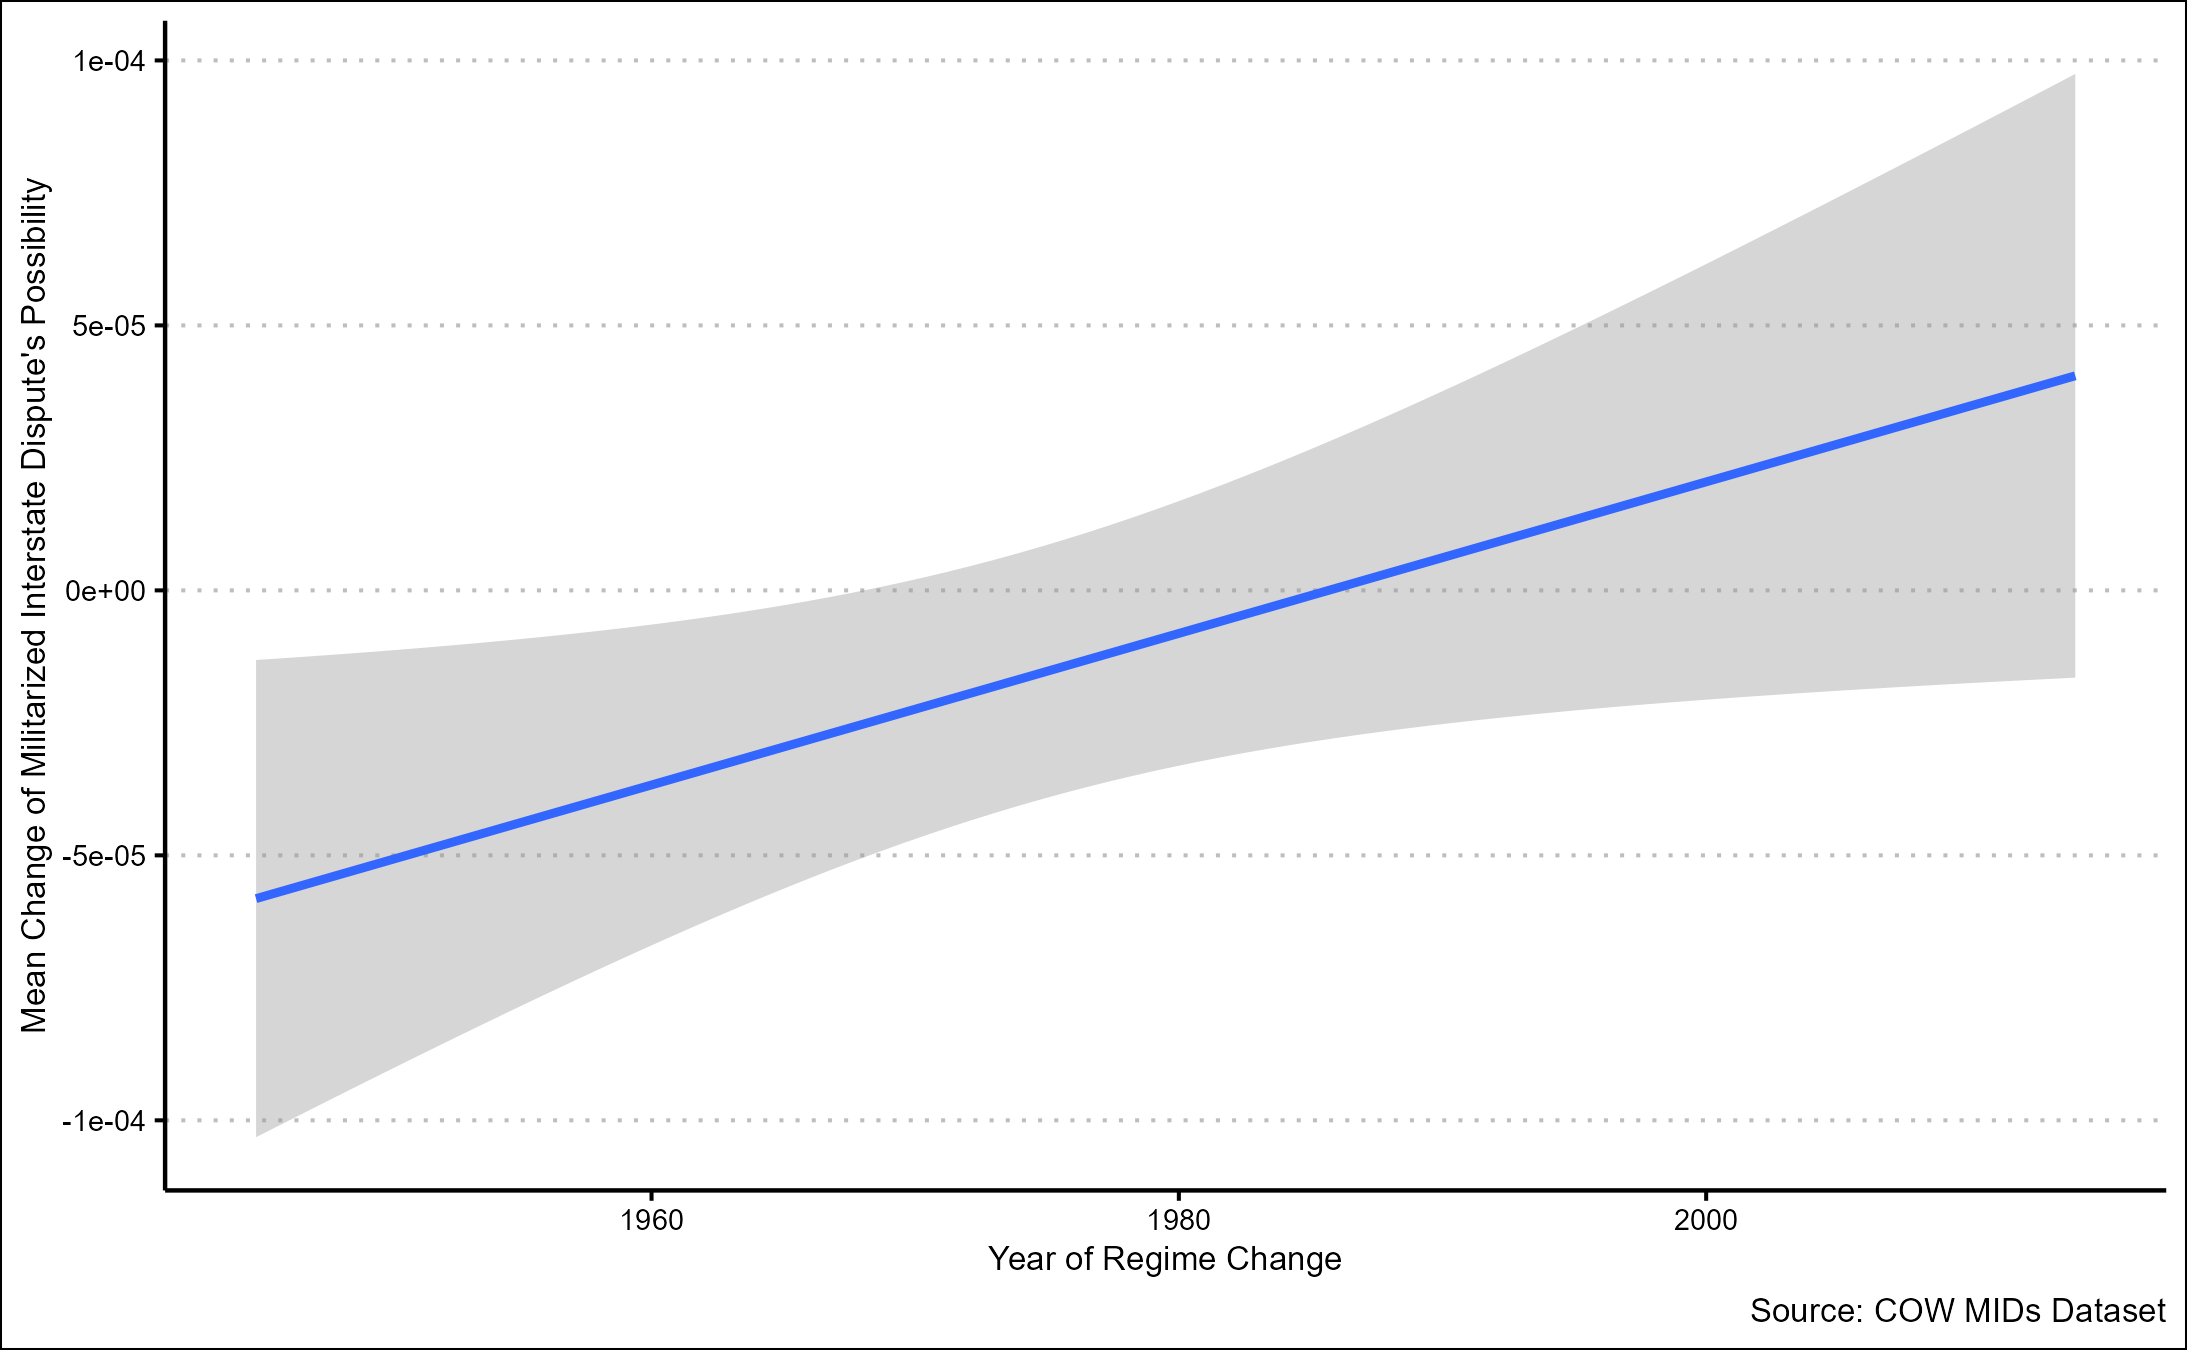
\includegraphics[width=1\linewidth]{paratrend.png}
\caption{Parallel Trend With Regime Change as Treatment Effect\label{fig:paratrend}}
\end{figure}
\noindent From figure~\ref{fig:paratrend}, we can observe a clear pattern in average change of possibility of militarized interstate disputes, and the mean change is significantly different in pre-treatment periods between dyads with regime change and dyads without regime change.  (results see Appendix~\ref{app4}) Given the violation of parallel trend assumption, the identification in causing the difference-in-differences---differences between treatment and control group in terms of changes due to regime change---can hardly be distinguished. 
\\Even though parallel trend assumption is violated, we can still look into how the causal identification is "approximately" correct instead of "exactly" correct. \parencite{rambachan_2023_a} By extrapolating pre-existing difference which violates parallel trend, \textcite{rambachan_2023_a} suggest that allow the ATT to deviate non-linearly from pre-existing trend and impose a restriction $M$ to limit the deviation within a confidence interval. Robustness can still be generated by conducting sensitivity analysis of ATT to conclude how bad the post-treatment violation of parallel trends can be.

\subsection{Two-Way Fixed Effects Model}
\begin{table}[hptb]
    \centering
\begin{tabular}{lcccc}
   \tabularnewline \midrule \midrule
   Dependent Variable: & \multicolumn{4}{c}{Militarized Interstate Dispute Onset}\\
   Model:                                & (1)            & (2)                     & (3)                            & (4)\\  
   \midrule
   \emph{Variables}\\
   Regime Change                           & -0.0001        & -0.0003                 & -0.0003                        & 0.0012\\   
                                         & (0.0004)       & (0.0004)                & (0.0004)                       & (0.0020)\\   
   Foreign Policy Similarity                               & 0.0090$^{***}$ & 0.0060                  & -0.0088$^{**}$                 & -0.0064\\   
                                         & (0.0021)       & (0.0077)                & (0.0043)                       & (0.0047)\\   
   Regime Change $\times$ \\Foreign Policy Similarity          & 0.0030         & 0.0022                  & 0.0029                         & -0.0166\\   
                                         & (0.0025)       & (0.0019)                & (0.0021)                       & (0.0103)\\   
   Strategic Rivalry                        &                & 0.1566$^{***}$          & 0.1850$^{***}$                 & 0.1911$^{***}$\\   
                                         &                & (0.0226)                & (0.0163)                       & (0.0181)\\   
   Alliance                              &                & -0.0065                 & 0.0098$^{**}$                  & 0.0073\\   
                                         &                & (0.0086)                & (0.0049)                       & (0.0053)\\   
   Major Power                                 &                & 0.0066$^{**}$           & -0.0034                        & -0.0035\\   
                                         &                & (0.0033)                & (0.0105)                       & (0.0105)\\   
   Distance                               &                & $1.12\times 10^{-5}$    & $-2.09\times 10^{-6}$$^{***}$  & $-1.96\times 10^{-6}$$^{***}$\\    
                                         &                & ($1.65\times 10^{-5}$)  & ($3.63\times 10^{-7}$)         & ($3.65\times 10^{-7}$)\\    
   $Distance^2$                        &                & $-5.65\times 10^{-10}$  & $9.34\times 10^{-11}$$^{***}$  & $8.52\times 10^{-11}$$^{***}$\\    
                                         &                & ($7.2\times 10^{-10}$)  & ($1.86\times 10^{-11}$)        & ($1.85\times 10^{-11}$)\\    
   Trade                            &                & -0.0002                 & -0.0002                        & -0.0002\\   
                                         &                & (0.0016)                & (0.0011)                       & (0.0011)\\   
   Economic Development                            &                & -0.0030$^{***}$         & -0.0011                        & -0.0011\\   
                                         &                & (0.0008)                & (0.0010)                       & (0.0010)\\   
   National Military Capability                              &                & -0.0008                 & -0.0054$^{***}$                & -0.0056$^{***}$\\   
                                         &                & (0.0014)                & (0.0011)                       & (0.0011)\\   
   Regime Change $\times$ \\Strategic Rivalry   &                &                         &                                & -0.0294\\   
                                         &                &                         &                                & (0.0248)\\   
   Regime Change $\times$ \\Alliance         &                &                         &                                & 0.0201$^{*}$\\   
                                         &                &                         &                                & (0.0108)\\   
   Regime Change $\times$ \\Distance          &                &                         &                                & $-7.65\times 10^{-7}$\\    
                                         &                &                         &                                & ($4.94\times 10^{-7}$)\\    
   Regime Change $\times$ \\$Distance^2$    &                &                         &                                & $4.75\times 10^{-11}$$^{*}$\\    
                                         &                &                         &                                & ($2.61\times 10^{-11}$)\\    
   Regime Change $\times$ \\National Military Capability         &                &                         &                                & 0.0006\\   
                                         &                &                         &                                & (0.0005)\\   
   \midrule
   \emph{Fixed-effects}\\
   ccode1                                & Yes            &                         & Yes                            & Yes\\  
   ccode2                                & Yes            &                         & Yes                            & Yes\\  
   year                                  & Yes            & Yes                     & Yes                            & Yes\\  
   id                                    &                & Yes                     &                                & \\  
   \midrule
   \emph{Fit statistics}\\
   Observations                          & 583,166        & 448,180                 & 448,180                        & 448,180\\  
   R$^2$                                 & 0.02226        & 0.16284                 & 0.08000                        & 0.08035\\  
   Within R$^2$                          & 0.00112        & 0.01236                 & 0.05915                        & 0.05950\\  
   \midrule \midrule
   \multicolumn{5}{l}{\emph{Signif. Codes: ***: 0.01, **: 0.05, *: 0.1}}\\
\end{tabular}
    \caption{Two-way Fixed Effect Regression Model}
    \label{twfe}
\end{table}

From table~\ref{twfe}, I only include key explanatory variables in model 1 and the standard error is clustered by controlling nation state $i$, nation state $j$ and time. Later in model 2, I add all the control variables into the regression model with individual standard error that is clustered by dyads and time. Model 3 has the same formula as model 2 but using model 1's standard error. For model 4, I include interactive terms between treatment variale and control variables that have statistical significance from model 4. 
\\Firstly, the Two-way fixed effect models gain more robustness from using clustered standard error that controls fixed effect of nation state $i$, nation state $j$ and time. Key explanatory variable, foreign policy similarity, gains statistical significance and reduce its standard error. Control variable such as strategic rivalry, alliance, distance, national military capability also become significant in model 4.
\\However, key causal identifications, regime change and interaction between regime change and foreign policy similarity, do not have statistical significance in any model. Regime change may have negative bias and regime change $\times$ foreign policy similarity may have positive bias from cross-sectional endogeneity and violations of parallel trend. Neither hypothesis reject the null and two-way fixed effect regression results fail to identify any casusal relationship between regime change and militarized interstate dispute onsets. It indicates that regime change may expose dyads with more possibility of military interstate disputes and when regime change takes place, dyads that share less similarity in foreign policy may have more possibility to suffer military interstate disputes.

\subsection{Event Study and Difference-in-Differences}
To further examine the causal identification of key explanatory variables, I examine the leads and lags up to 10 periods for each key explanatory variable through event study.

\begin{figure}[!hptb]
\centering
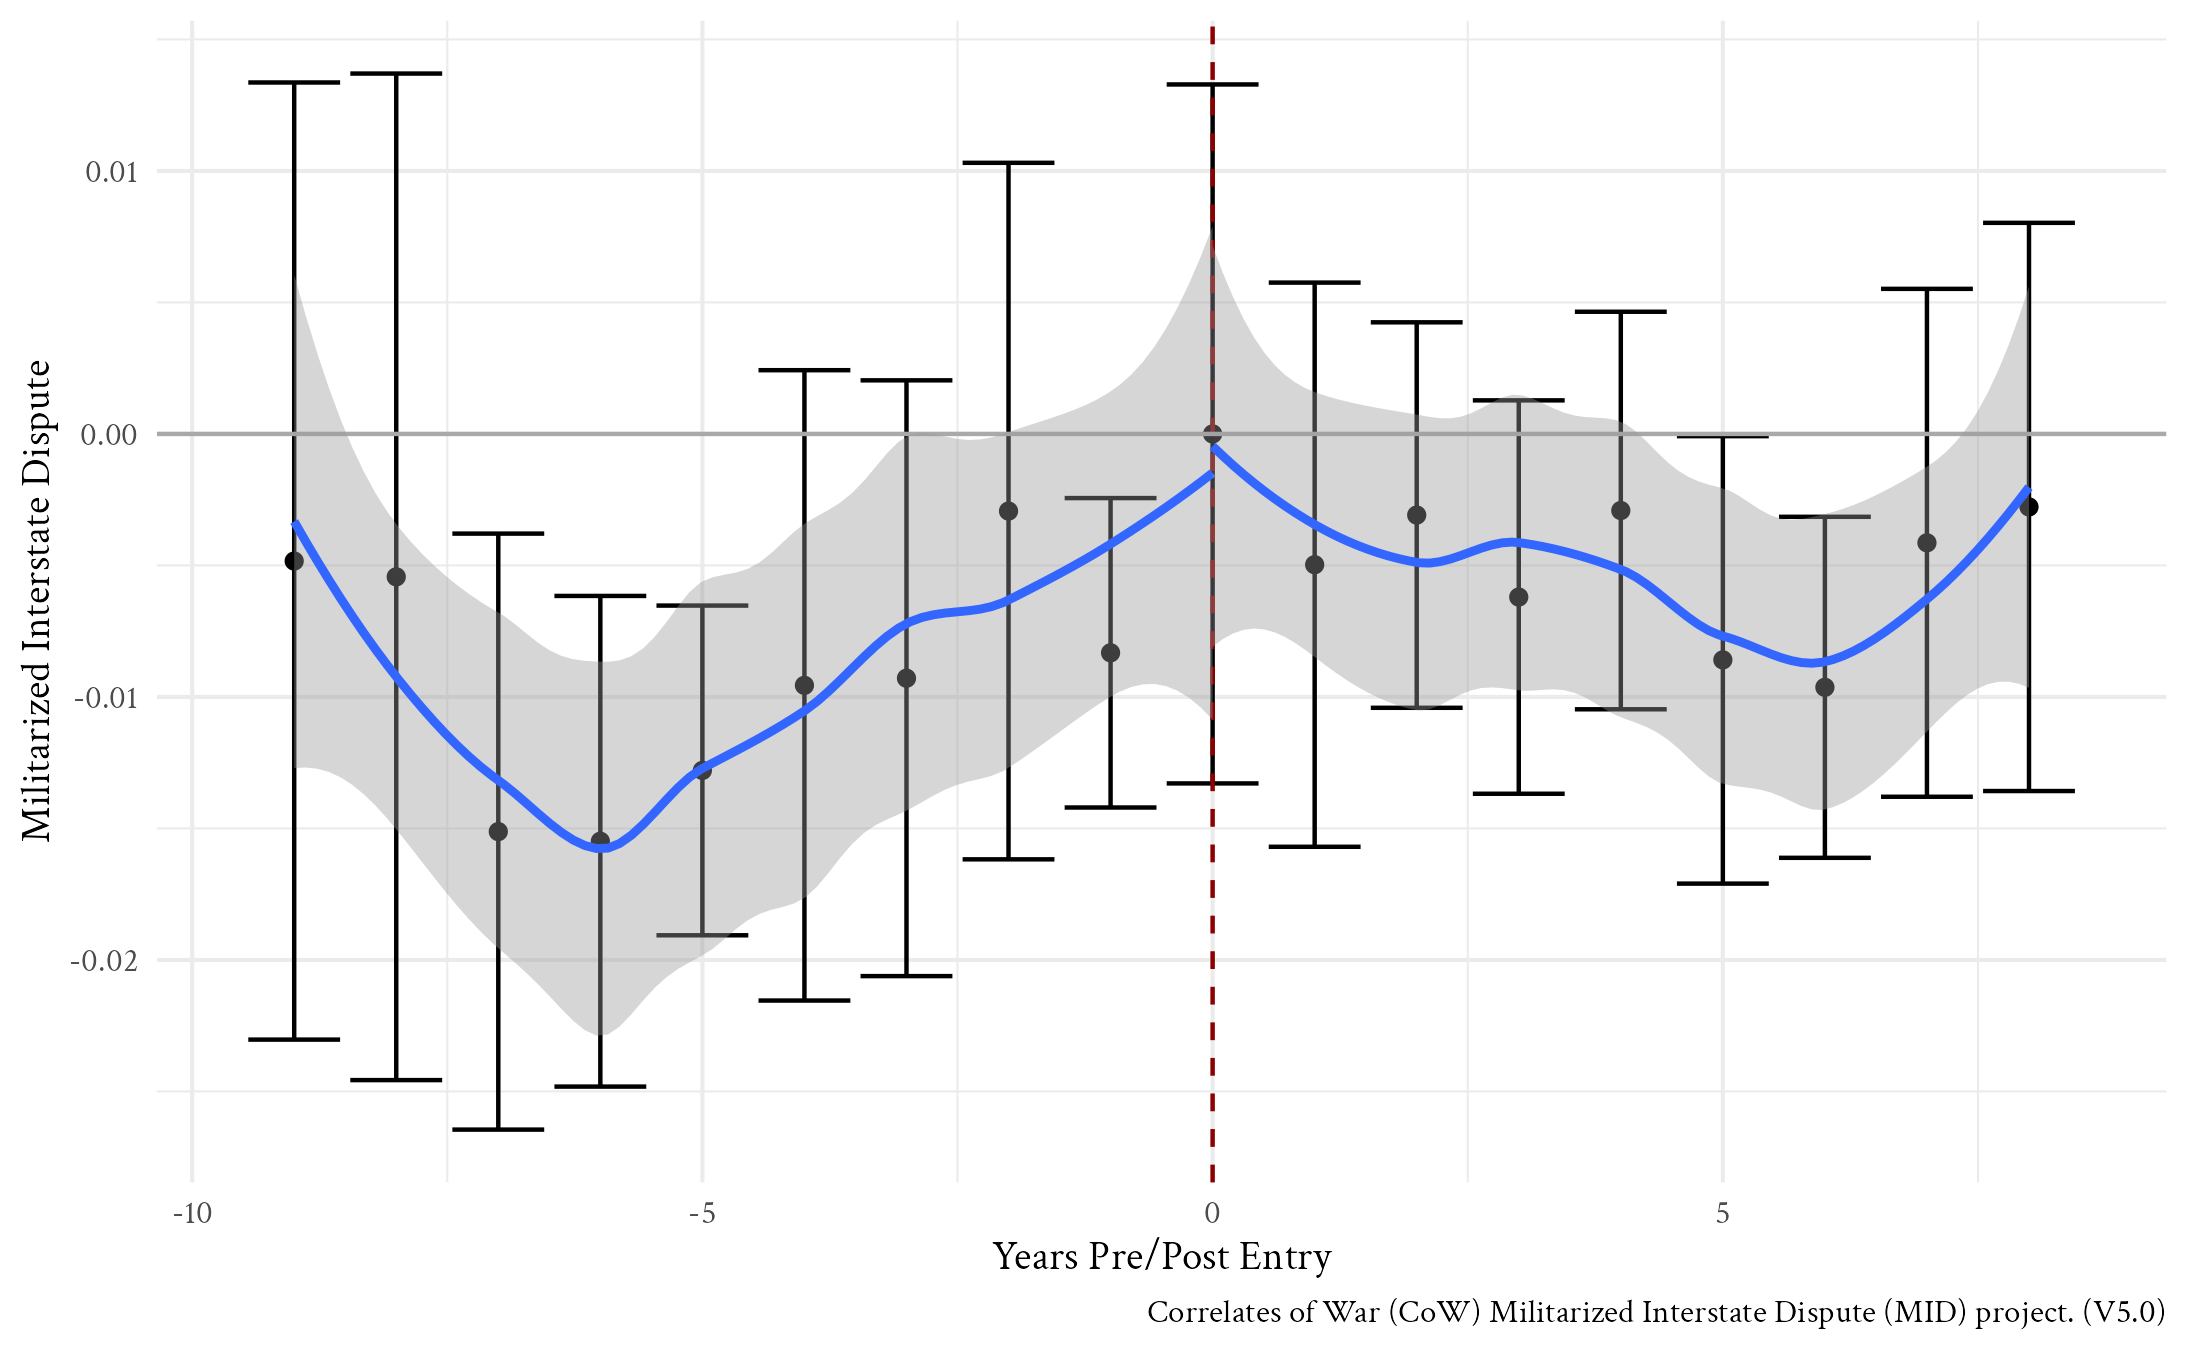
\includegraphics[width=1\linewidth]{leadslags.png}
\caption{\label{fig:leadslags}Leads and Lags for Regime Change}
\end{figure}

\begin{figure}[!hptb]
\centering
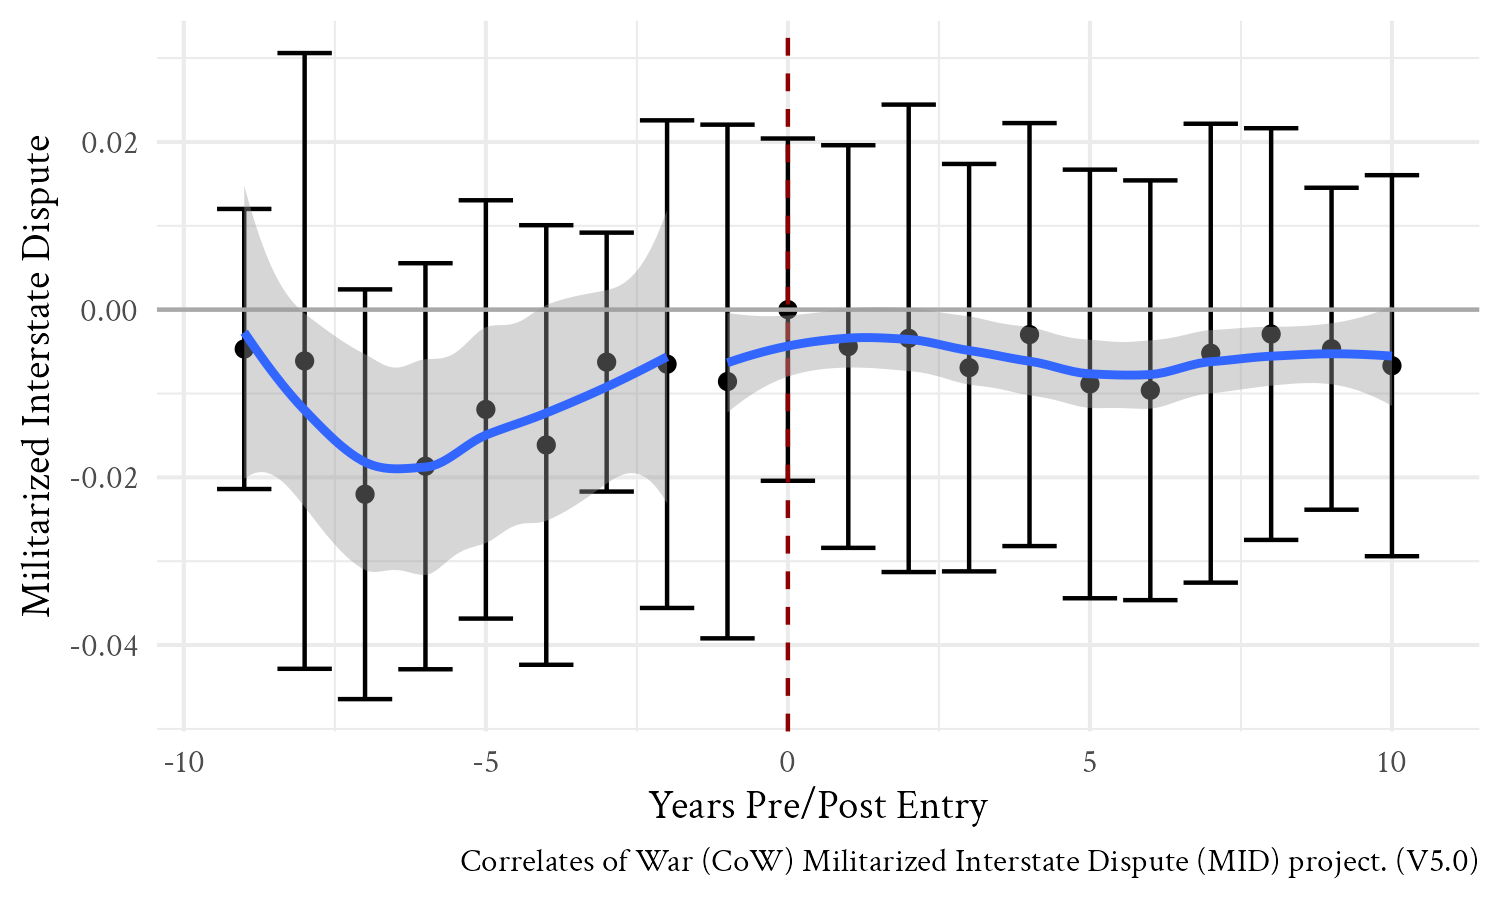
\includegraphics[width=1\linewidth]{leadslags_fpsi.png}
\caption{\label{fig:fpsi}Leads and Lags for Regime Change $\times$ Foreign Policy Similarity}
\end{figure}
\noindent From the event study plots, we are able to further validate a violation of parallel trends. For instance figure~\ref{fig:leadslags}, the ATT of regime change has significant change before leads 5 and the ATT of regime change $\times$ foreign policy similarity has a obvious turn between leads 10 and leads 5 from figure~\ref{fig:fpsi}. Moreover, figure~\ref{fig:fpsi}, I place the threshold at leads 1 in lieu of a observed jump from leads 1 to lags 0. It indicates a unknown shock that results in such jump. Therefore, the event study results are unable to derive a robust ATT from both key explanatory variables for causal identification in lags.

\begin{figure}[!hptb]
\centering
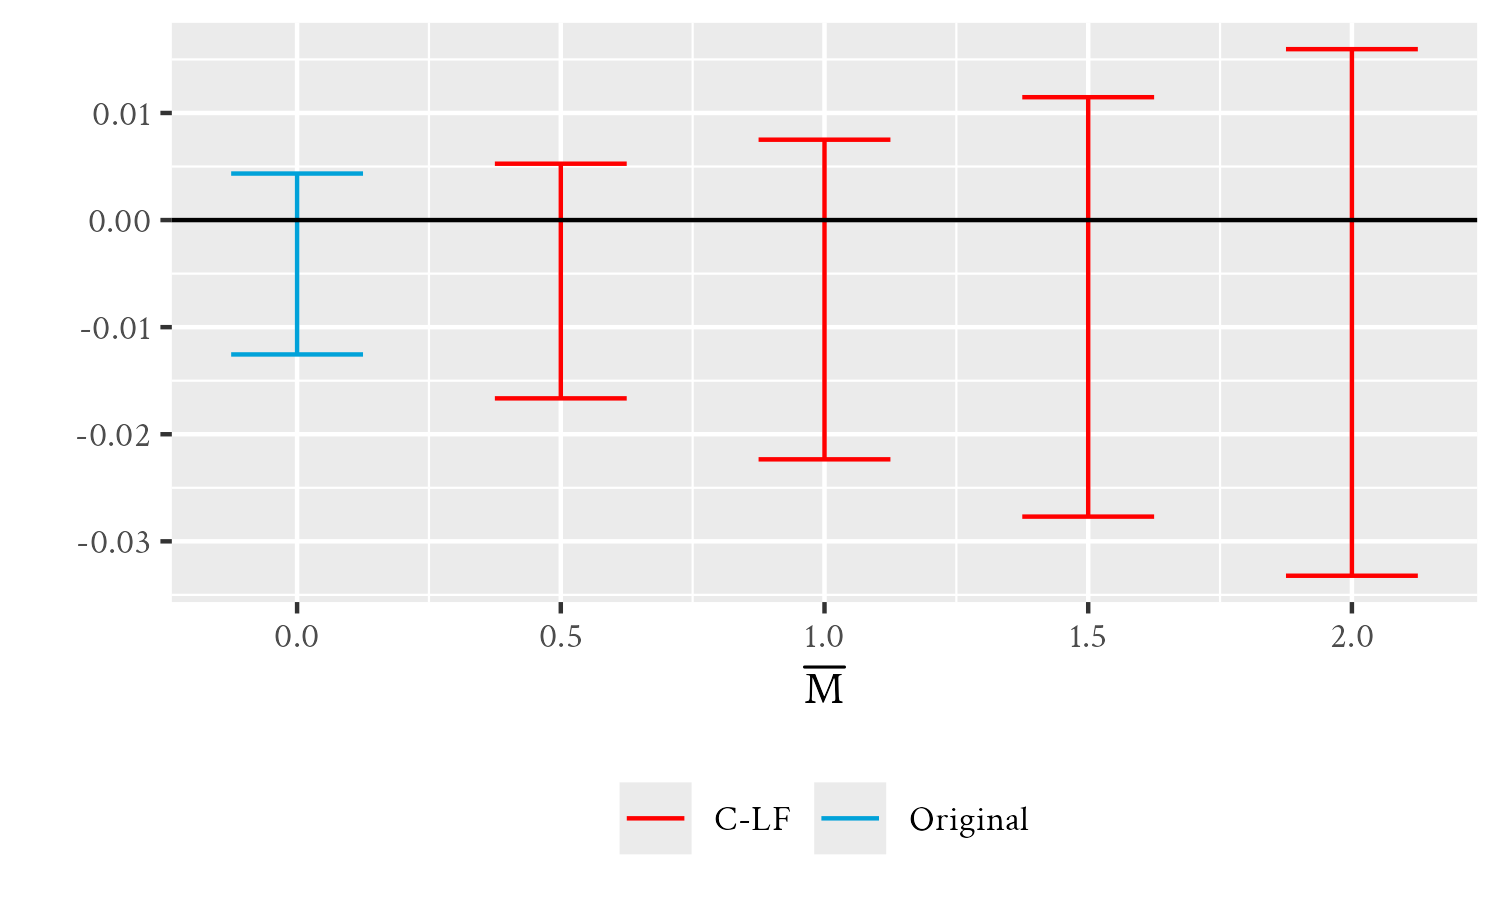
\includegraphics[width=1\linewidth]{similarity_rg.png}
\caption{\label{fig:simi_rg}Sensitivity Plot With Relative Magnitudes for Regime Change}
\end{figure}

\begin{figure}[!hptb]
\centering
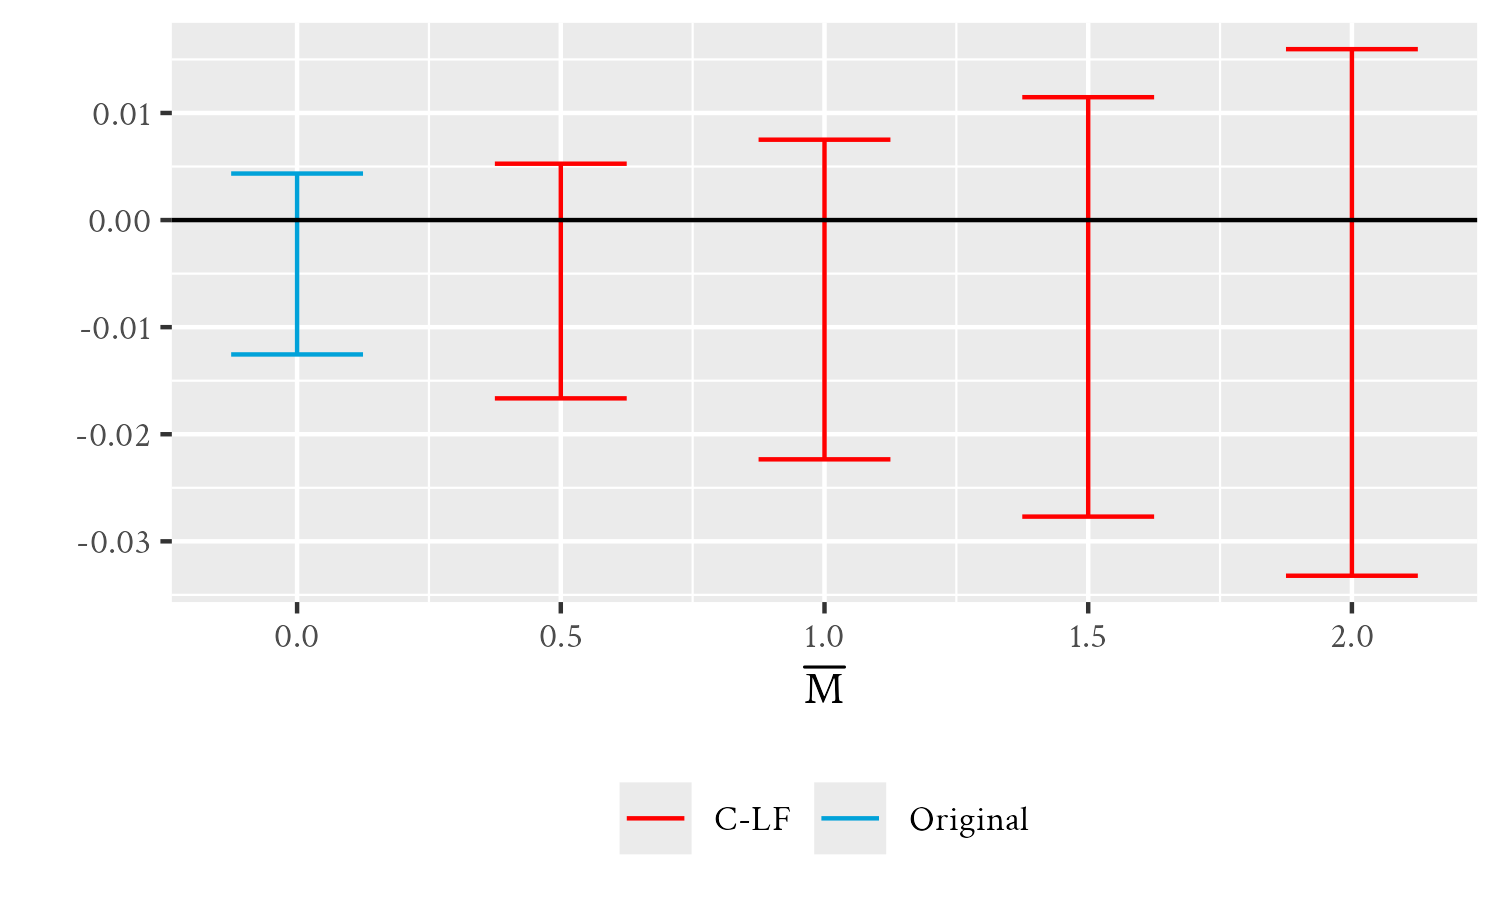
\includegraphics[width=1\linewidth]{similarity_fpsi.png}
\caption{\label{fig:simi_fpsi}Sensitivity Plot With Relative Magnitudes for Regime Change $\times$ Foreign Policy Similarity}
\end{figure}
\noindent In terms of sensitivity test, from figure~\ref{fig:simi_rg} and figure~\ref{fig:simi_fpsi} we observe an acceptable deviation to capture causal trends from pre-existing trends at the level of restriction $\overline{M}$ vary across 0. As the restriction increases and the confidence level gets larger, the ATT of key explanatory variables increase more in negative side than in positive side. It also exposes a issue that it is hard to distinguish the direction of bias from parallel trend and cross-sectional endogeneity. Even though the negative is captured more than at positive side, there is no confidence to infer any causal relationship from the similarity test. (see \ref{app5} for ATT's confidence interval)

%--- Section ---%
xw\section{Conclusions}
Even though there is no robust causal inference from this research, the conclusion can still be drawn from that there may exist a causal relationship that dyads with regime change may have greater possibility to encounter less possibility of militarized interstate dispute onsets, because from the sensitivity test result shows that negative ATT is captured more in the confidence interval. Same rationale applied to a possible case exists when dyads that share less similarity in foreign policy are more likely to engage in a militarized interstate dispute due to regime change. 
\\The reason why this study fails to identify a clear causal relationship is that fundamental pre-assumptions is violated and unable to be addressed. The sensitivity test does not address the issue that parallel trend assumption is violated. What's more, the cross-sectional endogeneity is also causing bias to ATT. A robust conclusion that can be infered from this research is that the ATT of regime change and of regime change $\times$ foreign policy similarity is likely to be negative regardless of parallel trends being violated.
\\ The problem of heterogeneity and endogeneity may result from loss of information in lieu of dyadic unit. Nation state $i$ and nation state $j$ may contain rich information, e.g., less indicators for differences among dyads and more indicators for differences among nation states, about their decision to engage in militarized interstate disputes. Moreover, in this case, unit specific trend analysis can be used to examine endogeneity problems if parallel trend is violated. 

%-------------------------------------------
% References
%-------------------------------------------

% Print bibliography
\printbibliography




%-------------------------------------------
% Appendix
%-------------------------------------------
% Activate the appendix in the doc
% from here on sections are numerated with capital letters 
%\appendix

% Change equation numbering format to be sequential within sections in the appendix
\renewcommand\theequation{\Alph{section}\arabic{equation}} % Redefine equation numbering format
\counterwithin*{equation}{section} % Number equations within sections
\renewcommand\thefigure{\Alph{section}\arabic{figure}} % Redefine equation numbering format
\counterwithin*{figure}{section} % Number equations within sections
\renewcommand\thetable{\Alph{section}\arabic{table}} % Redefine equation numbering format
\counterwithin*{table}{section} % Number equations within sections

\begin{appendices}

%--- Section ---%
\section{Appendix}
\subsection{Time Span}\label{app1}
From \ref{fig:regime1816} we can see that Major Powerity of the dyad-year regime change happened after 1940s. 
\begin{figure}[!hptb]
\centering
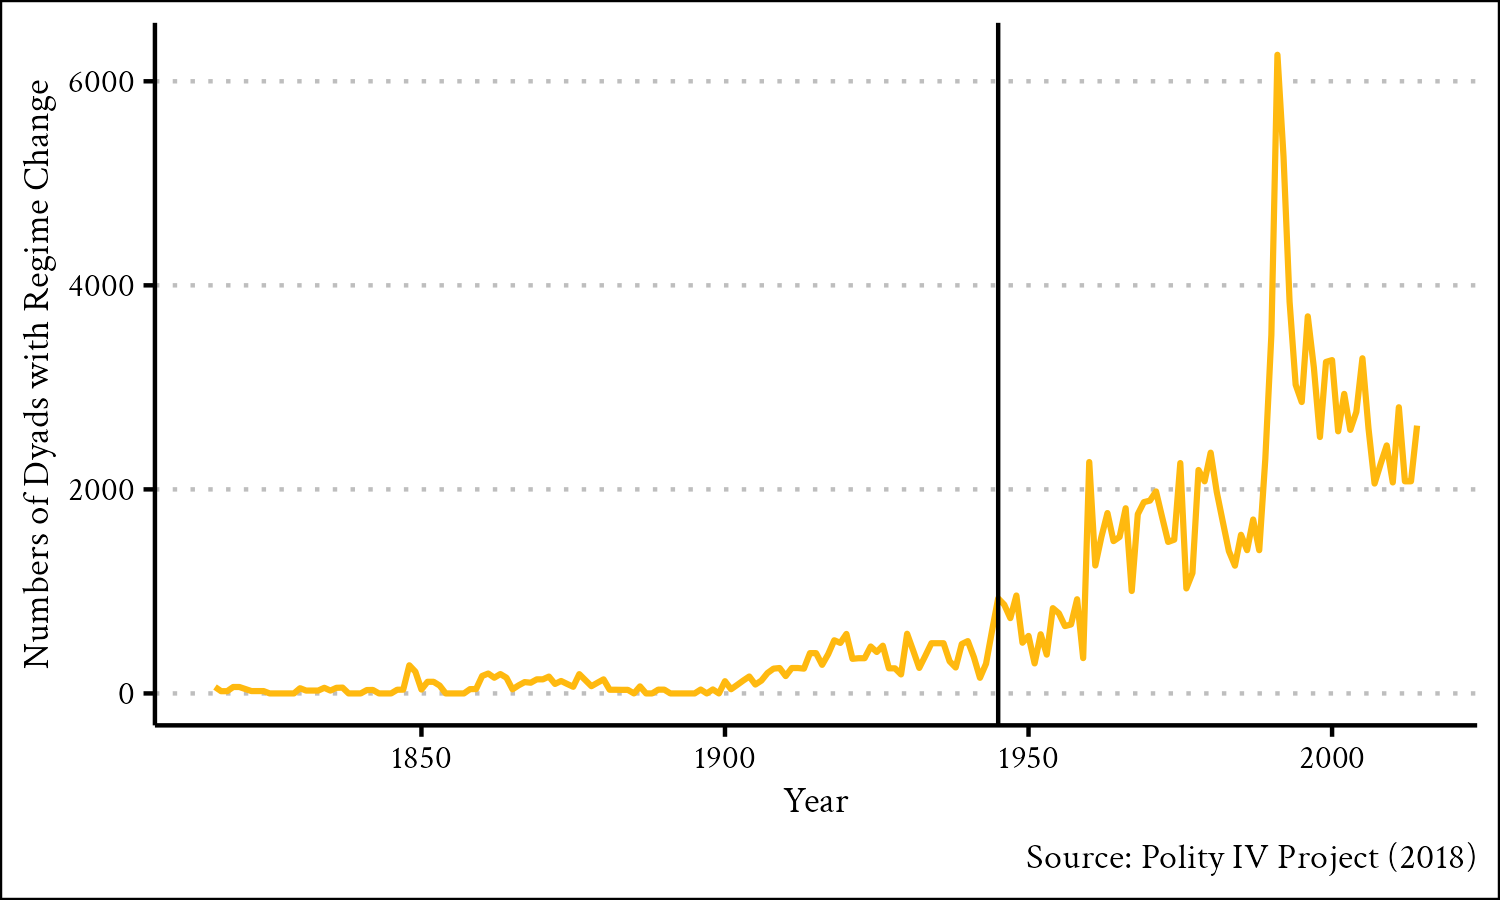
\includegraphics[width=1\linewidth]{regime1816.png}
\caption{\label{fig:regime1816}Numbers of Dyads with Regime Change, from 1816 to 2014.}
\end{figure}

\subsection{Effect Size}\label{app2}
The estimated effect size is $0.08\%$ and the minimum detected effect is 0.0065. The data sample will be sufficient to detect the anticipated impact.

\begin{table}[!hptb]
\centering
\caption{Effect Size F-Test\label{efsize}}
\begin{tabular}{lc}
   \tabularnewline \midrule \midrule
   Dependent Variable: & MID onset\\  
   Model:              & (1)\\  
   \midrule
   \emph{Variables}\\
   Regime Change         & $-8.81\times 10^{-5}$\\    
                       & (0.0004)\\   
   \midrule
   \emph{Fixed-effects}\\
   Year                & Yes\\  
   State $i$              & Yes\\  
   State $j$              & Yes\\  
   \midrule
   \emph{Fit statistics}\\
   Observations        & 583,166\\  
   R$^2$               & 0.02116\\  
   Within R$^2$        & $3.36\times 10^{-7}$\\   
   \midrule \midrule
   \multicolumn{2}{l}{\emph{Clustered (year) standard-errors in parentheses}}\\
   \multicolumn{2}{l}{\emph{Signif. Codes: ***: 0.01, **: 0.05, *: 0.1}}\\
\end{tabular}
\end{table}

\begin{figure}[!hptb]
\centering
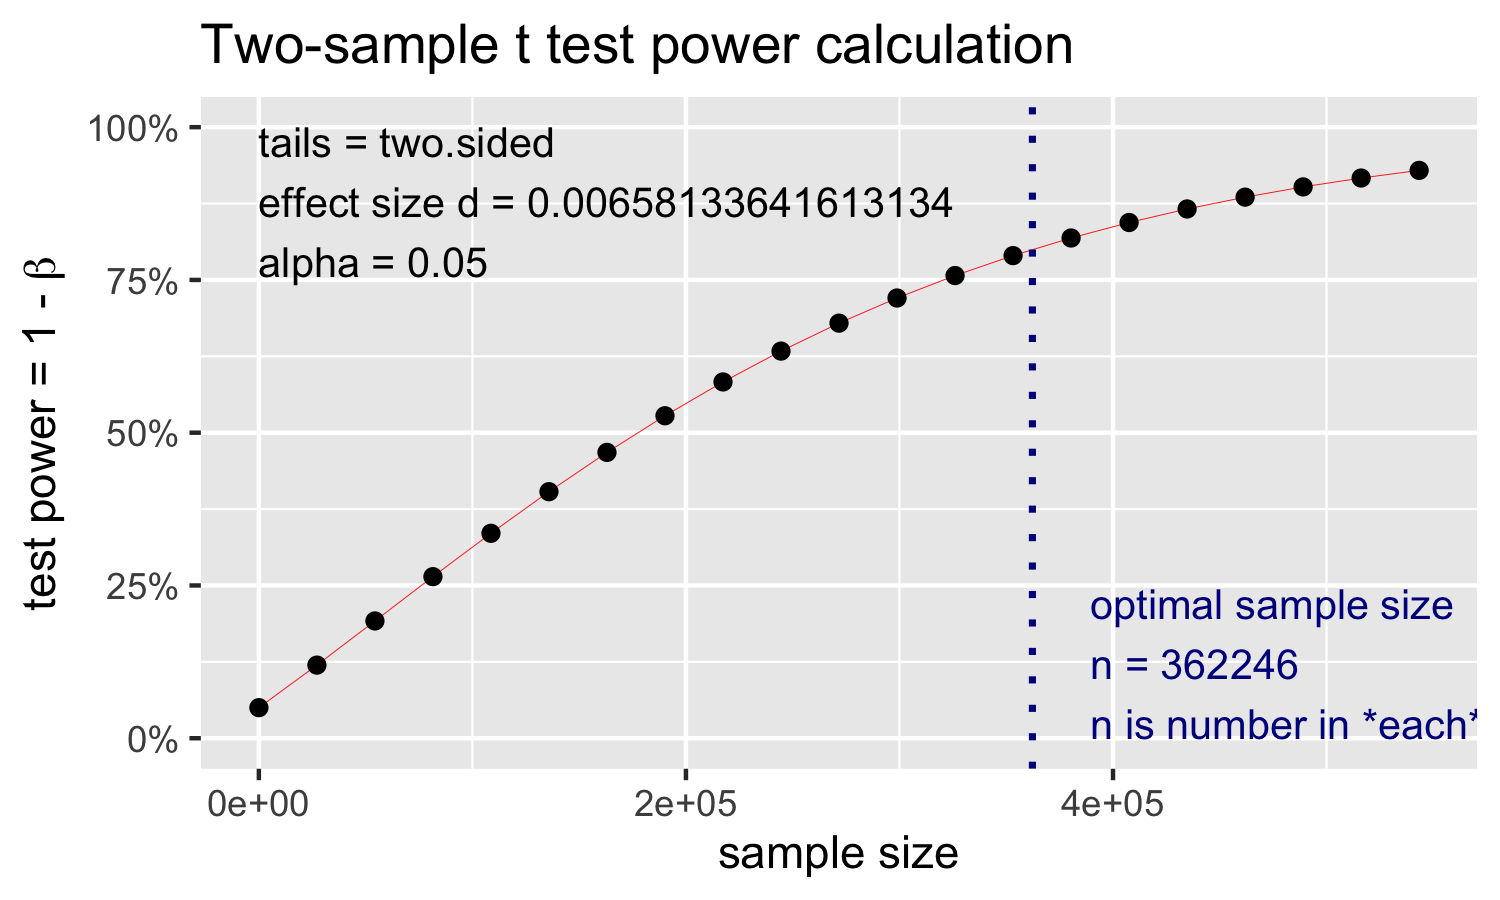
\includegraphics[width=1\linewidth]{mde.png}
\caption{\label{mde}}
\end{figure}

\subsection{Cross-sectional Endogeneity Test}\label{app3}
\begin{table}[!hptb]
\centering
\caption{Cross-sectional Endogeneity Test\label{cset}}
\begin{tabular}{lcccccc}
   \tabularnewline \midrule \midrule
   Dependent Variable: & \multicolumn{6}{c}{Entry Year}\\
   Model:         & (1)             & (2)                     & (3)             & (4)             & (5)             & (6)\\  
   \midrule
   \emph{Variables}\\
   Constant       & 1,941.6$^{***}$ & 1,971.2$^{***}$         & 1,974.6$^{***}$ & 1,974.1$^{***}$ & 1,974.2$^{***}$ & 1,973.7$^{***}$\\   
                  & (1.388)         & (0.1488)                & (0.1437)        & (0.1398)        & (0.1399)        & (0.1360)\\   
   Economic Development     & 1.823$^{***}$   &                         &                 &                 &                 &   \\   
                  & (0.0801)        &                         &                 &                 &                 &   \\   
   Trade     &                 & -0.0004$^{***}$         &                 &                 &                 &   \\   
                  &                 & ($5.03\times 10^{-5}$)  &                 &                 &                 &   \\   
   National Military Capability       &                 &                         & -102.2$^{***}$  &                 &                 &   \\   
                  &                 &                         & (5.631)         &                 &                 &   \\   
   Major Power Power          &                 &                         &                 & -7.341$^{***}$  &                 &   \\   
                  &                 &                         &                 & (0.5695)        &                 &   \\   
   Alliance       &                 &                         &                 &                 & -9.103$^{***}$  &   \\   
                  &                 &                         &                 &                 & (0.6209)        &   \\   
   Strategic Rivalry        &                 &                         &                 &                 &                 & -16.03$^{***}$\\   
                  &                 &                         &                 &                 &                 & (2.642)\\   
   \midrule
   \emph{Fit statistics}\\
   Observations   & 16,646          & 13,781                  & 17,118          & 17,118          & 17,118          & 17,118\\  
   R$^2$          & 0.03019         & 0.00436                 & 0.01887         & 0.00962         & 0.01240         & 0.00215\\  
   Adjusted R$^2$ & 0.03013         & 0.00428                 & 0.01881         & 0.00956         & 0.01235         & 0.00209\\  
   \midrule \midrule
   \multicolumn{7}{l}{\emph{IID standard-errors in parentheses}}\\
   \multicolumn{7}{l}{\emph{Signif. Codes: ***: 0.01, **: 0.05, *: 0.1}}\\
\end{tabular}
\end{table}
\newpage


\subsection{Parallel Trends Analysis}\label{app4}
\begin{table}[!hptb]
\centering
\caption{Parallel Trend F-Test\label{paratrend}}
\begin{tabular}{lc}
   \tabularnewline \midrule \midrule
   Dependent Variable: & treatyr\\  
   Model:              & (1)\\  
   \midrule
   \emph{Variables}\\
   Constant            & 1,973.7$^{***}$\\   
                       & (0.1359)\\   
   avg\_mid            & 255.7$^{***}$\\   
                       & (76.82)\\   
   \midrule
   \emph{Fit statistics}\\
   Observations        & 17,109\\  
   R$^2$               & 0.00065\\  
   Adjusted R$^2$      & 0.00059\\  
   \midrule \midrule
   \multicolumn{2}{l}{\emph{IID standard-errors in parentheses}}\\
   \multicolumn{2}{l}{\emph{Signif. Codes: ***: 0.01, **: 0.05, *: 0.1}}\\
\end{tabular}
\end{table}
\newpage

\subsection{Event Study}\label{app5}
\begin{table}[!hptb]
\centering
\begin{tabular}{rrrllr}
  \hline
 & lb & ub & method & Delta & Mbar \\ 
  \hline
1 & -0.02 & 0.01 & C-LF & DeltaRM & 0.50 \\ 
  2 & -0.02 & 0.01 & C-LF & DeltaRM & 1.00 \\ 
  3 & -0.03 & 0.01 & C-LF & DeltaRM & 1.50 \\ 
  4 & -0.03 & 0.02 & C-LF & DeltaRM & 2.00 \\ 
   \hline
\end{tabular}
    \caption{Sensitivity Table With Relative Magnitudes for Regime Change}
    \label{tab:rg}
\end{table}
\begin{table}[!hptb]
\centering
\begin{tabular}{rrrllr}
  \hline
 & lb & ub & method & Delta & Mbar \\ 
  \hline
1 & -0.02 & 0.04 & C-LF & DeltaRM & 0.50 \\ 
  2 & -0.04 & 0.06 & C-LF & DeltaRM & 1.00 \\ 
  3 & -0.06 & 0.08 & C-LF & DeltaRM & 1.50 \\ 
  4 & -0.08 & 0.10 & C-LF & DeltaRM & 2.00 \\ 
   \hline
\end{tabular}
    \caption{Sensitivity Table With Relative Magnitudes for Regime Change $\times$ Foreign Policy Similarity}
    \label{tab:fpsi}
\end{table}


%--- Section ---%
\end{appendices}
\end{document}